\documentclass[11pt]{article}            % Report class in 11 points
\parindent0pt  \parskip10pt             % make block paragraphs
\usepackage{graphicx}
\usepackage{listings}
\graphicspath{ {images/} }
\usepackage{graphicx} %  graphics header file
\begin{document}
\begin{titlepage}
    \centering
  \vfill
    
\includegraphics[width=8cm]{uni_logo.png} \\ 
	\vskip2cm
    {\bfseries\Large
	Data Structures and algorythm  \\ (CS09203)\\
	
	\vskip2cm
	Lab Report 
	 
	\vskip2cm
	}    

\begin{center}
\begin{tabular}{ l l  } 

Name: & MuhammadTalhaKhalid \\ 
Registration \#: &CSU-S16-135\\ 
Lab Report \#: & 4 \\ 
 Dated:& 21-04-2018\\ 
Submitted To:& Mr. Usman Ahmed\\ 

 %\hline
\end{tabular}
\end{center}
    \vfill
    The University of Lahore, Islamabad Campus\\
Department of Computer Science \& Information Technology
\end{titlepage}


    
    {\bfseries\Large
\centering
	Experiment \# 4 \\

Data Handling  by Link List\\
	
	}    
 \vskip1cm
 \textbf {Objective}\\  To understand How to Insert and Delete Data using Link list .
 
 \textbf {Software Tool} \\
1. Linux Ubuntu \\
2. G++\\
3. Miktext editor \\

\section{Theory }              
In this experiment we learn how to handle our data using  link listing using Link list , Create new node and move address of 1st node to second location When we enter our data it create a new node the 1st node has our data and second has its address and the last one is NULL and so on \\
It has 4 rules:\\
1.	Nodes.\\
2.	*Head .\\ 
3.	*Tail.\\ 
4.	*New Node.\\ 

\section{Task}  
\subsection{Procedure: Task 1 }     

\begin{figure*}
\centering
  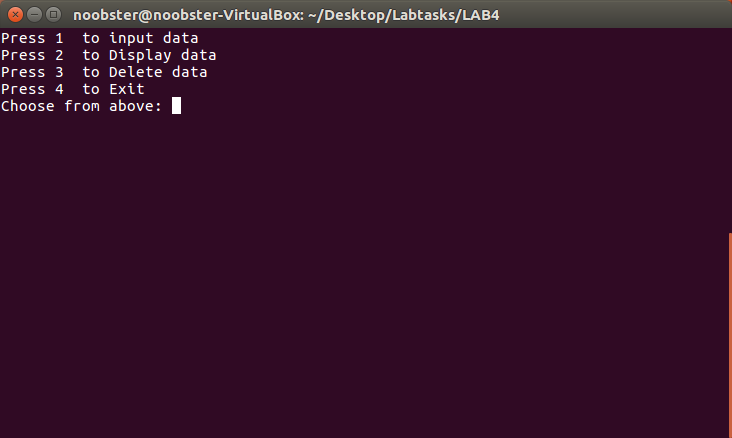
\includegraphics[width=12cm,height=6cm,keepaspectratio]{1.png}
\caption{Main menu of my program}
\label{Figure:1}    
  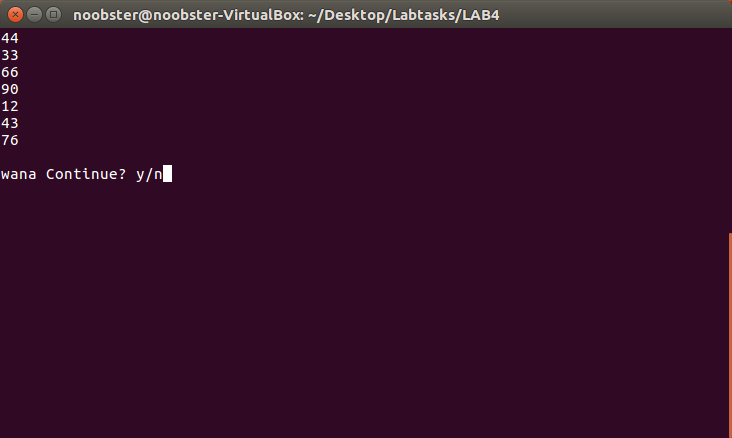
\includegraphics[width=12cm,height=6cm,keepaspectratio]{2.png}
\caption{enter 7 number  into link list}
\label{Figure:2}   
\end{figure*}
In this We eter our data into link list the link list create node and enter our data and moves its address to next node and the other node is now null to delete it it search for the data you enter into the nodes and if data is not found it will go to next node and so on\ 
\subsection{Procedure: Task 2 }   
\begin{lstlisting}[language=C++]
#include<iostream>
#include<stdio.h>
#include <unistd.h>
#include<cstdlib>
using namespace std;
class Node {
public:
	int Data;
 Node *Next; 
};
class linklist {
public:
	Node *Head;
	Node *Tail;
	Node *NewNode;
	linklist() {
		Head=Tail=NULL;
		NewNode=NULL;
	}
	 void AddNode(int num) {
     NewNode=new Node;
     NewNode->Data=num;
     cout<<"Sucesfully entered "<<NewNode->Data<<"\n";
     if(Head==NULL){
     	Head=NewNode;
     	Tail=NewNode;
     }
     else {
     		Tail->Next=NewNode;
     		Tail=Tail->Next;
     	}
	 }
	 void Display(){
	 	Node *temp;
	 	temp=Head;
	 	while(temp!=NULL) {
	 		cout<<temp->Data<<endl;
	 		temp=temp->Next;
	 	}
	 }

	 void Delete(int num) {
	 	Node *temp;
	 	Node *prev;
	 	//Previous=Head;
	 	if(Head==NULL) {
	 		cerr<<"Node is Empty!! \n";
	 		return;
	 	}else {
	 		if(Head->Data==num) {
	 			Head=Head->Next;
	 			
	 		} else { 
	 			temp=Head;
	 			
	 			while(temp!=NULL && temp->Data!=num){
	 				prev=temp;
	 				temp=temp->Next;
	 			} //while
	 			
	 			prev->Next=temp->Next;
	 			delete temp; 			
	 		}//if
	 	}//wada if
	 }
};
void menu() {
	cout<<"Press 1  to input data \n";
	cout<<"Press 2  to Display data \n";
	cout<<"Press 3  to Delete data \n";
	cout<<"Press 4  to Exit \n";
}
int Choice;
string Schoice="y";
int main() 
{
	int num;
linklist LI;
do {
system("clear");
menu();
cout<<"Choose from above: ";
cin>>Choice;
switch (Choice) {
	case 1:
	system("clear");
	do {
		cout<<"Enter a number: ";
		cin>>num;
		LI.AddNode(num);
		cout<<"\nwana Continue? y/n";
		cin>>Schoice;
	}while(Schoice!="n");
	break;

	case 2:
	system("clear");
	do {
		LI.Display();
		cout<<"\nwana Continue? y/n";
		cin>>Schoice;
	}while(Schoice!="n");
	break;
	case 3:
	system("clear");
	do {
		LI.Display();
		cout<<"\nEnter a number you wana delete: ";
		cin>>num;
		LI.Delete(num);
		cout<<"\nwana Continue? y/n";
		cin>>Schoice;
	}while(Schoice!="n");
	break;
	}
}while(Choice!=4);
return 0;
}
\end{lstlisting}
\begin{figure*}
\section{Conclusion: }
So we cone to a conclusion that  how to use link list basic concept of nodes and Pointers and how nodes work   and basic concept about data structures \ \  \\
\section{Output: }
\centering
  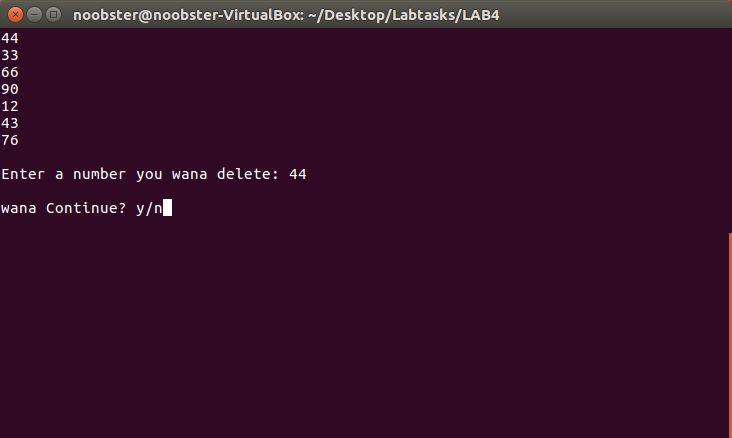
\includegraphics[width=12cm,height=6cm,keepaspectratio]{3.png}
\caption{Display output of my Stored Data}
\label{Figure:3}   
 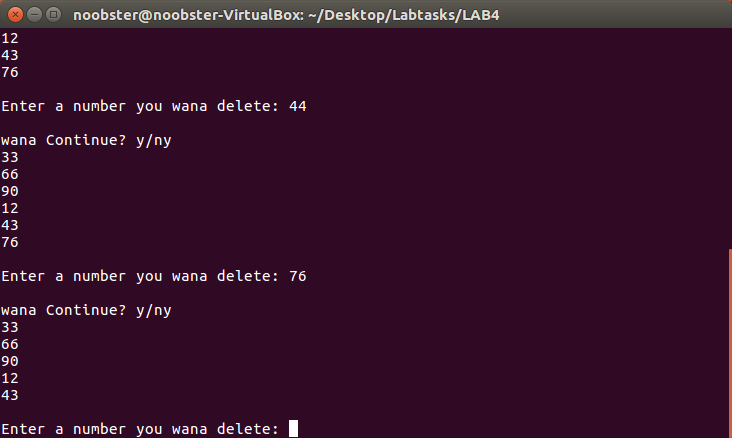
\includegraphics[width=12cm,height=6cm,keepaspectratio]{4.png}
\caption{Remove 44 and 76 from my link list}
\label{Figure:4}
\end{figure*}

\end{document}                          % The required last line
